\documentclass[1p]{elsarticle_modified}
%\bibliographystyle{elsarticle-num}

%\usepackage[colorlinks]{hyperref}
%\usepackage{abbrmath_seonhwa} %\Abb, \Ascr, \Acal ,\Abf, \Afrak
\usepackage{amsfonts}
\usepackage{amssymb}
\usepackage{amsmath}
\usepackage{amsthm}
\usepackage{scalefnt}
\usepackage{amsbsy}
\usepackage{kotex}
\usepackage{caption}
\usepackage{subfig}
\usepackage{color}
\usepackage{graphicx}
\usepackage{xcolor} %% white, black, red, green, blue, cyan, magenta, yellow
\usepackage{float}
\usepackage{setspace}
\usepackage{hyperref}

\usepackage{tikz}
\usetikzlibrary{arrows}

\usepackage{multirow}
\usepackage{array} % fixed length table
\usepackage{hhline}

%%%%%%%%%%%%%%%%%%%%%
\makeatletter
\renewcommand*\env@matrix[1][\arraystretch]{%
	\edef\arraystretch{#1}%
	\hskip -\arraycolsep
	\let\@ifnextchar\new@ifnextchar
	\array{*\c@MaxMatrixCols c}}
\makeatother %https://tex.stackexchange.com/questions/14071/how-can-i-increase-the-line-spacing-in-a-matrix
%%%%%%%%%%%%%%%

\usepackage[normalem]{ulem}

\newcommand{\msout}[1]{\ifmmode\text{\sout{\ensuremath{#1}}}\else\sout{#1}\fi}
%SOURCE: \msout is \stkout macro in https://tex.stackexchange.com/questions/20609/strikeout-in-math-mode

\newcommand{\cancel}[1]{
	\ifmmode
	{\color{red}\msout{#1}}
	\else
	{\color{red}\sout{#1}}
	\fi
}

\newcommand{\add}[1]{
	{\color{blue}\uwave{#1}}
}

\newcommand{\replace}[2]{
	\ifmmode
	{\color{red}\msout{#1}}{\color{blue}\uwave{#2}}
	\else
	{\color{red}\sout{#1}}{\color{blue}\uwave{#2}}
	\fi
}

\newcommand{\Sol}{\mathcal{S}} %segment
\newcommand{\D}{D} %diagram
\newcommand{\A}{\mathcal{A}} %arc


%%%%%%%%%%%%%%%%%%%%%%%%%%%%%5 test

\def\sl{\operatorname{\textup{SL}}(2,\Cbb)}
\def\psl{\operatorname{\textup{PSL}}(2,\Cbb)}
\def\quan{\mkern 1mu \triangleright \mkern 1mu}

\theoremstyle{definition}
\newtheorem{thm}{Theorem}[section]
\newtheorem{prop}[thm]{Proposition}
\newtheorem{lem}[thm]{Lemma}
\newtheorem{ques}[thm]{Question}
\newtheorem{cor}[thm]{Corollary}
\newtheorem{defn}[thm]{Definition}
\newtheorem{exam}[thm]{Example}
\newtheorem{rmk}[thm]{Remark}
\newtheorem{alg}[thm]{Algorithm}

\newcommand{\I}{\sqrt{-1}}
\begin{document}

%\begin{frontmatter}
%
%\title{Boundary parabolic representations of knots up to 8 crossings}
%
%%% Group authors per affiliation:
%\author{Yunhi Cho} 
%\address{Department of Mathematics, University of Seoul, Seoul, Korea}
%\ead{yhcho@uos.ac.kr}
%
%
%\author{Seonhwa Kim} %\fnref{s_kim}}
%\address{Center for Geometry and Physics, Institute for Basic Science, Pohang, 37673, Korea}
%\ead{ryeona17@ibs.re.kr}
%
%\author{Hyuk Kim}
%\address{Department of Mathematical Sciences, Seoul National University, Seoul 08826, Korea}
%\ead{hyukkim@snu.ac.kr}
%
%\author{Seokbeom Yoon}
%\address{Department of Mathematical Sciences, Seoul National University, Seoul, 08826,  Korea}
%\ead{sbyoon15@snu.ac.kr}
%
%\begin{abstract}
%We find all boundary parabolic representation of knots up to 8 crossings.
%
%\end{abstract}
%\begin{keyword}
%    \MSC[2010] 57M25 
%\end{keyword}
%
%\end{frontmatter}

%\linenumbers
%\tableofcontents
%
\newcommand\colored[1]{\textcolor{white}{\rule[-0.35ex]{0.8em}{1.4ex}}\kern-0.8em\color{red} #1}%
%\newcommand\colored[1]{\textcolor{white}{ #1}\kern-2.17ex	\textcolor{white}{ #1}\kern-1.81ex	\textcolor{white}{ #1}\kern-2.15ex\color{red}#1	}

{\Large $\underline{12a_{1181}~(K12a_{1181})}$}

\setlength{\tabcolsep}{10pt}
\renewcommand{\arraystretch}{1.6}
\vspace{1cm}\begin{tabular}{m{100pt}>{\centering\arraybackslash}m{274pt}}
\multirow{5}{120pt}{
	\centering
	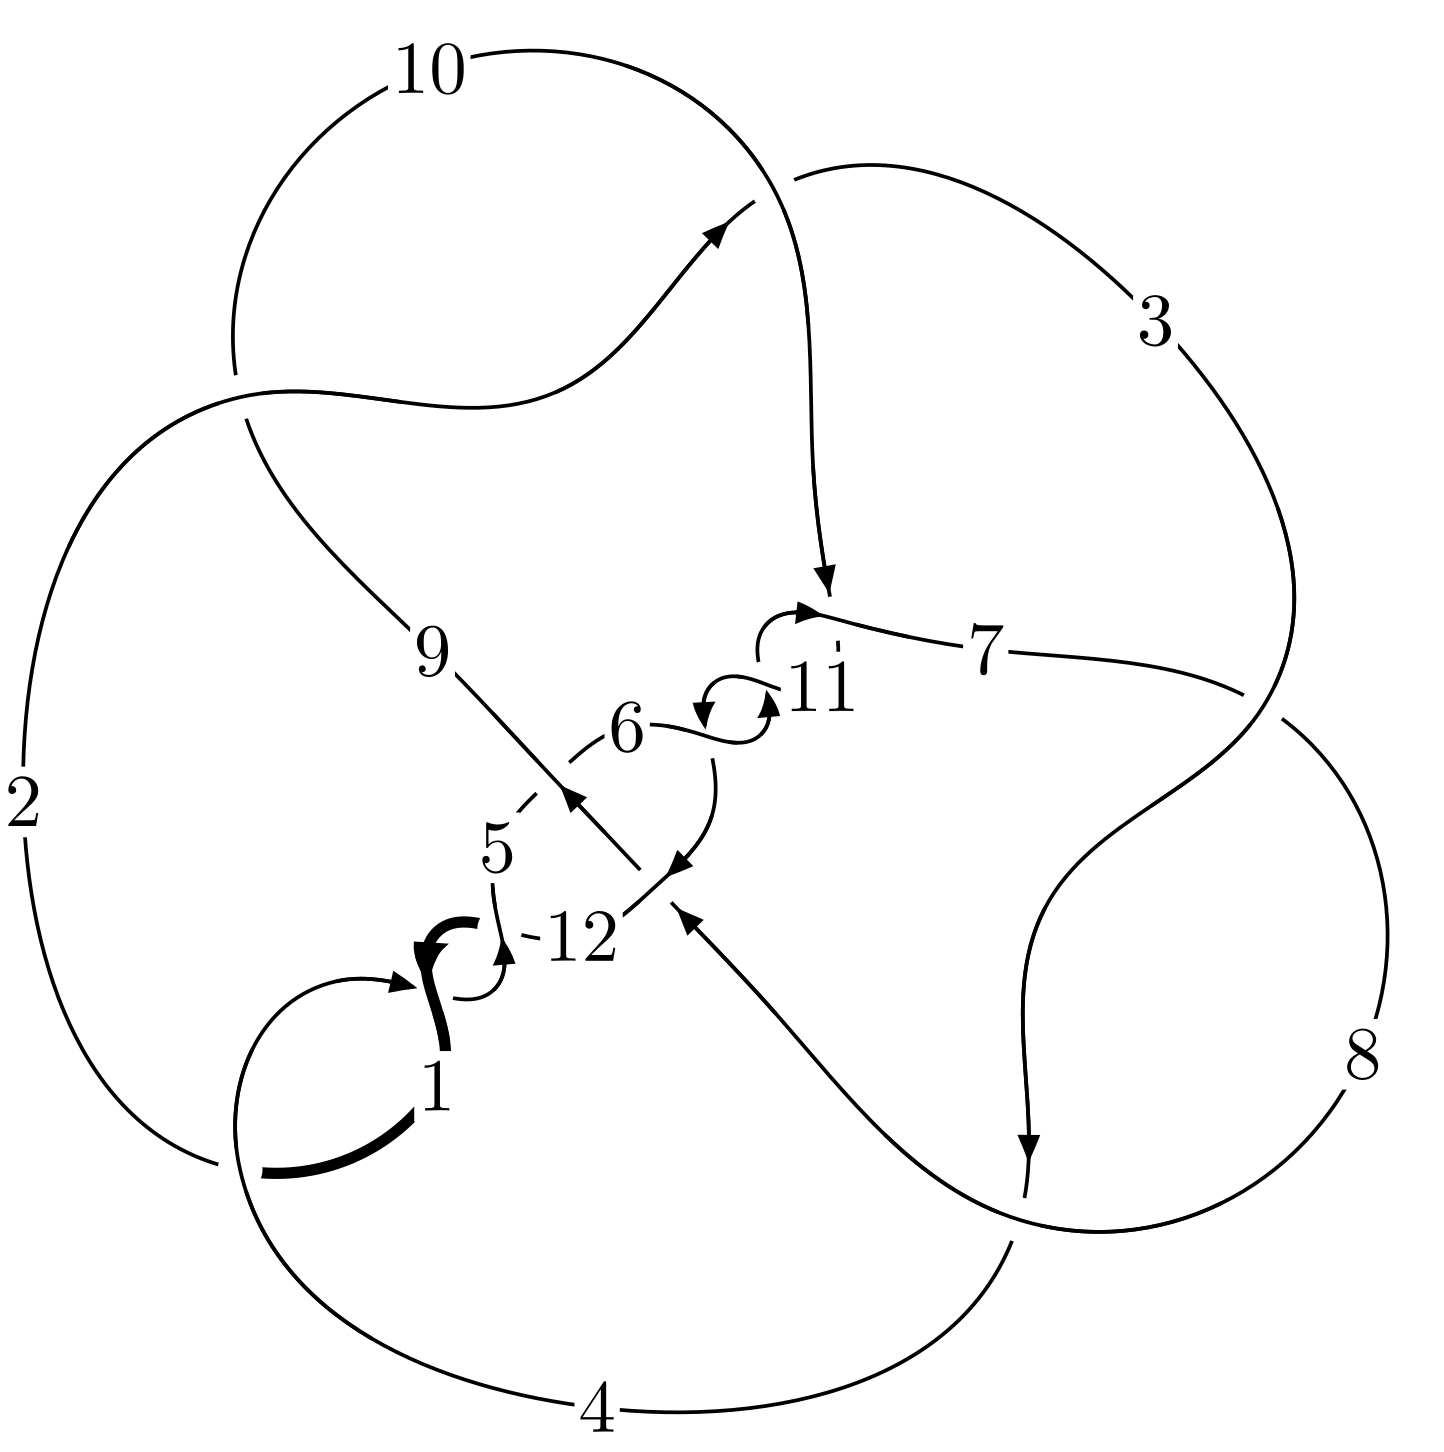
\includegraphics[width=112pt]{../../../GIT/diagram.site/Diagrams/png/1982_12a_1181.png}\\
\ \ \ A knot diagram\footnotemark}&
\allowdisplaybreaks
\textbf{Linearized knot diagam} \\
\cline{2-2}
 &
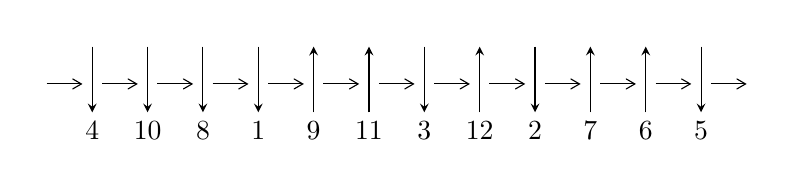
\begin{tikzpicture}[x=20pt, y=17pt]
	% nodes
	\node (C0) at (0, 0) {};
	\node (C1) at (1, 0) {};
	\node (C1U) at (1, +1) {};
	\node (C1D) at (1, -1) {4};

	\node (C2) at (2, 0) {};
	\node (C2U) at (2, +1) {};
	\node (C2D) at (2, -1) {10};

	\node (C3) at (3, 0) {};
	\node (C3U) at (3, +1) {};
	\node (C3D) at (3, -1) {8};

	\node (C4) at (4, 0) {};
	\node (C4U) at (4, +1) {};
	\node (C4D) at (4, -1) {1};

	\node (C5) at (5, 0) {};
	\node (C5U) at (5, +1) {};
	\node (C5D) at (5, -1) {9};

	\node (C6) at (6, 0) {};
	\node (C6U) at (6, +1) {};
	\node (C6D) at (6, -1) {11};

	\node (C7) at (7, 0) {};
	\node (C7U) at (7, +1) {};
	\node (C7D) at (7, -1) {3};

	\node (C8) at (8, 0) {};
	\node (C8U) at (8, +1) {};
	\node (C8D) at (8, -1) {12};

	\node (C9) at (9, 0) {};
	\node (C9U) at (9, +1) {};
	\node (C9D) at (9, -1) {2};

	\node (C10) at (10, 0) {};
	\node (C10U) at (10, +1) {};
	\node (C10D) at (10, -1) {7};

	\node (C11) at (11, 0) {};
	\node (C11U) at (11, +1) {};
	\node (C11D) at (11, -1) {6};

	\node (C12) at (12, 0) {};
	\node (C12U) at (12, +1) {};
	\node (C12D) at (12, -1) {5};
	\node (C13) at (13, 0) {};

	% arrows
	\draw[->,>={angle 60}]
	(C0) edge (C1) (C1) edge (C2) (C2) edge (C3) (C3) edge (C4) (C4) edge (C5) (C5) edge (C6) (C6) edge (C7) (C7) edge (C8) (C8) edge (C9) (C9) edge (C10) (C10) edge (C11) (C11) edge (C12) (C12) edge (C13) ;	\draw[->,>=stealth]
	(C1U) edge (C1D) (C2U) edge (C2D) (C3U) edge (C3D) (C4U) edge (C4D) (C5D) edge (C5U) (C6D) edge (C6U) (C7U) edge (C7D) (C8D) edge (C8U) (C9U) edge (C9D) (C10D) edge (C10U) (C11D) edge (C11U) (C12U) edge (C12D) ;
	\end{tikzpicture} \\
\hhline{~~} \\& 
\textbf{Solving Sequence} \\ \cline{2-2} 
 &
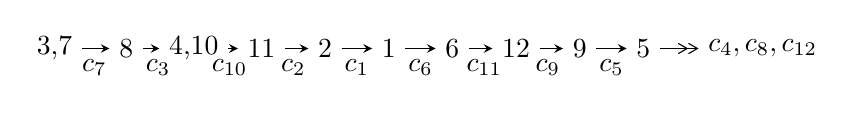
\begin{tikzpicture}[x=23pt, y=7pt]
	% node
	\node (A0) at (-1/8, 0) {3,7};
	\node (A1) at (1, 0) {8};
	\node (A2) at (33/16, 0) {4,10};
	\node (A3) at (25/8, 0) {11};
	\node (A4) at (33/8, 0) {2};
	\node (A5) at (41/8, 0) {1};
	\node (A6) at (49/8, 0) {6};
	\node (A7) at (57/8, 0) {12};
	\node (A8) at (65/8, 0) {9};
	\node (A9) at (73/8, 0) {5};
	\node (C1) at (1/2, -1) {$c_{7}$};
	\node (C2) at (3/2, -1) {$c_{3}$};
	\node (C3) at (21/8, -1) {$c_{10}$};
	\node (C4) at (29/8, -1) {$c_{2}$};
	\node (C5) at (37/8, -1) {$c_{1}$};
	\node (C6) at (45/8, -1) {$c_{6}$};
	\node (C7) at (53/8, -1) {$c_{11}$};
	\node (C8) at (61/8, -1) {$c_{9}$};
	\node (C9) at (69/8, -1) {$c_{5}$};
	\node (A10) at (11, 0) {$c_{4},c_{8},c_{12}$};

	% edge
	\draw[->,>=stealth]	
	(A0) edge (A1) (A1) edge (A2) (A2) edge (A3) (A3) edge (A4) (A4) edge (A5) (A5) edge (A6) (A6) edge (A7) (A7) edge (A8) (A8) edge (A9) ;
	\draw[->>,>={angle 60}]	
	(A9) edge (A10);
\end{tikzpicture} \\ 

\end{tabular} \\

\footnotetext{
The image of knot diagram is generated by the software ``\textbf{Draw programme}" developed by Andrew Bartholomew(\url{http://www.layer8.co.uk/maths/draw/index.htm\#Running-draw}), where we modified some parts for our purpose(\url{https://github.com/CATsTAILs/LinksPainter}).
}\phantom \\ \newline 
\centering \textbf{Ideals for irreducible components\footnotemark of $X_{\text{par}}$} 
 
\begin{align*}
I^u_{1}&=\langle 
-14254847226477 u^{26}+36513086551233 u^{25}+\cdots+25218582104246 b+69411294847385,\\
\phantom{I^u_{1}}&\phantom{= \langle  }a-1,\;u^{27}-2 u^{26}+\cdots- u+1\rangle \\
I^u_{2}&=\langle 
1.54251\times10^{20} u^{23}-1.34594\times10^{20} u^{22}+\cdots+4.03018\times10^{21} b+1.66567\times10^{20},\\
\phantom{I^u_{2}}&\phantom{= \langle  }2.09874\times10^{23} u^{23}+2.15950\times10^{23} u^{22}+\cdots+7.08424\times10^{25} a-6.56169\times10^{25},\;u^{24}-7 u^{22}+\cdots-17 u+44\rangle \\
I^u_{3}&=\langle 
-2706 u^{15}+399 u^{14}+\cdots+2389 b+1730,\;a+1,\\
\phantom{I^u_{3}}&\phantom{= \langle  }u^{16}-8 u^{14}+28 u^{12}- u^{11}-50 u^{10}+3 u^9+46 u^8-2 u^7-23 u^6- u^5+12 u^4+4 u^3-4 u^2- u+1\rangle \\
I^u_{4}&=\langle 
2.71133\times10^{33} u^{31}-1.79455\times10^{33} u^{30}+\cdots+1.73517\times10^{36} b+3.10903\times10^{35},\\
\phantom{I^u_{4}}&\phantom{= \langle  }-1.46619\times10^{42} u^{31}-3.55764\times10^{42} u^{30}+\cdots+1.02938\times10^{44} a-1.96344\times10^{44},\\
\phantom{I^u_{4}}&\phantom{= \langle  }u^{32}+u^{31}+\cdots+556 u+109\rangle \\
\\
\end{align*}
\raggedright * 4 irreducible components of $\dim_{\mathbb{C}}=0$, with total 99 representations.\\
\footnotetext{All coefficients of polynomials are rational numbers. But the coefficients are sometimes approximated in decimal forms when there is not enough margin.}
\newpage
\renewcommand{\arraystretch}{1}
\centering \section*{I. $I^u_{1}= \langle -1.43\times10^{13} u^{26}+3.65\times10^{13} u^{25}+\cdots+2.52\times10^{13} b+6.94\times10^{13},\;a-1,\;u^{27}-2 u^{26}+\cdots- u+1 \rangle$}
\flushleft \textbf{(i) Arc colorings}\\
\begin{tabular}{m{7pt} m{180pt} m{7pt} m{180pt} }
\flushright $a_{3}=$&$\begin{pmatrix}0\\u\end{pmatrix}$ \\
\flushright $a_{7}=$&$\begin{pmatrix}1\\0\end{pmatrix}$ \\
\flushright $a_{8}=$&$\begin{pmatrix}1\\u^2\end{pmatrix}$ \\
\flushright $a_{4}=$&$\begin{pmatrix}- u\\- u^3+u\end{pmatrix}$ \\
\flushright $a_{10}=$&$\begin{pmatrix}1\\0.565252 u^{26}-1.44786 u^{25}+\cdots+3.67612 u-2.75239\end{pmatrix}$ \\
\flushright $a_{11}=$&$\begin{pmatrix}0.565252 u^{26}-1.44786 u^{25}+\cdots+3.67612 u-1.75239\\0.565252 u^{26}-1.44786 u^{25}+\cdots+3.67612 u-2.75239\end{pmatrix}$ \\
\flushright $a_{2}=$&$\begin{pmatrix}u\\-0.317361 u^{26}+0.398104 u^{25}+\cdots-1.18714 u-0.565252\end{pmatrix}$ \\
\flushright $a_{1}=$&$\begin{pmatrix}0.0683574 u^{26}-0.219861 u^{25}+\cdots+1.08074 u+0.236618\\-0.398080 u^{26}+0.502028 u^{25}+\cdots-1.41938 u-0.718723\end{pmatrix}$ \\
\flushright $a_{6}=$&$\begin{pmatrix}-1.04115 u^{26}+1.62303 u^{25}+\cdots-4.19819 u-1.11991\\-1.60640 u^{26}+3.07090 u^{25}+\cdots-7.87431 u+0.632474\end{pmatrix}$ \\
\flushright $a_{12}=$&$\begin{pmatrix}-0.337903 u^{26}+0.670668 u^{25}+\cdots-1.19240 u-0.372411\\0.703245 u^{26}-0.952366 u^{25}+\cdots+3.00579 u+0.747502\end{pmatrix}$ \\
\flushright $a_{9}=$&$\begin{pmatrix}- u^2+1\\0.801869 u^{26}-1.98946 u^{25}+\cdots+4.55874 u-3.06975\end{pmatrix}$ \\
\flushright $a_{5}=$&$\begin{pmatrix}-0.0367769 u^{26}-0.0781692 u^{25}+\cdots-0.950528 u-0.0601984\\-0.265354 u^{26}+0.386964 u^{25}+\cdots-0.436197 u-0.0643596\end{pmatrix}$\\&\end{tabular}
\flushleft \textbf{(ii) Obstruction class $= -1$}\\~\\
\flushleft \textbf{(iii) Cusp Shapes $= -\frac{32741796610216}{12609291052123} u^{26}+\frac{41485402060855}{12609291052123} u^{25}+\cdots-\frac{145165804658306}{12609291052123} u-\frac{32798700861086}{12609291052123}$}\\~\\
\newpage\renewcommand{\arraystretch}{1}
\flushleft \textbf{(iv) u-Polynomials at the component}\newline \\
\begin{tabular}{m{50pt}|m{274pt}}
Crossings & \hspace{64pt}u-Polynomials at each crossing \\
\hline $$\begin{aligned}c_{1},c_{4},c_{12}\end{aligned}$$&$\begin{aligned}
&u^{27}-13 u^{26}+\cdots+240 u-16
\end{aligned}$\\
\hline $$\begin{aligned}c_{2},c_{3},c_{7}\\c_{9}\end{aligned}$$&$\begin{aligned}
&u^{27}-2 u^{26}+\cdots- u+1
\end{aligned}$\\
\hline $$\begin{aligned}c_{5},c_{8}\end{aligned}$$&$\begin{aligned}
&u^{27}- u^{25}+\cdots-4 u-1
\end{aligned}$\\
\hline $$\begin{aligned}c_{6},c_{10},c_{11}\end{aligned}$$&$\begin{aligned}
&u^{27}-15 u^{26}+\cdots+1792 u-128
\end{aligned}$\\
\hline
\end{tabular}\\~\\
\newpage\renewcommand{\arraystretch}{1}
\flushleft \textbf{(v) Riley Polynomials at the component}\newline \\
\begin{tabular}{m{50pt}|m{274pt}}
Crossings & \hspace{64pt}Riley Polynomials at each crossing \\
\hline $$\begin{aligned}c_{1},c_{4},c_{12}\end{aligned}$$&$\begin{aligned}
&y^{27}+23 y^{26}+\cdots+384 y-256
\end{aligned}$\\
\hline $$\begin{aligned}c_{2},c_{3},c_{7}\\c_{9}\end{aligned}$$&$\begin{aligned}
&y^{27}-24 y^{26}+\cdots-13 y-1
\end{aligned}$\\
\hline $$\begin{aligned}c_{5},c_{8}\end{aligned}$$&$\begin{aligned}
&y^{27}-2 y^{26}+\cdots+32 y-1
\end{aligned}$\\
\hline $$\begin{aligned}c_{6},c_{10},c_{11}\end{aligned}$$&$\begin{aligned}
&y^{27}+23 y^{26}+\cdots+49152 y-16384
\end{aligned}$\\
\hline
\end{tabular}\\~\\
\newpage\flushleft \textbf{(vi) Complex Volumes and Cusp Shapes}
$$\begin{array}{c|c|c}  
\text{Solutions to }I^u_{1}& \I (\text{vol} + \sqrt{-1}CS) & \text{Cusp shape}\\
 \hline 
\begin{aligned}
u &= \phantom{-}0.606808 + 0.696344 I \\
a &= \phantom{-}1.00000\phantom{ +0.000000I} \\
b &= -0.420246 + 0.658451 I\end{aligned}
 & \phantom{-}5.31904 - 1.53633 I & \phantom{-}0.97752 + 4.58695 I \\ \hline\begin{aligned}
u &= \phantom{-}0.606808 - 0.696344 I \\
a &= \phantom{-}1.00000\phantom{ +0.000000I} \\
b &= -0.420246 - 0.658451 I\end{aligned}
 & \phantom{-}5.31904 + 1.53633 I & \phantom{-}0.97752 - 4.58695 I \\ \hline\begin{aligned}
u &= -0.414460 + 0.742322 I \\
a &= \phantom{-}1.00000\phantom{ +0.000000I} \\
b &= -0.633985 + 0.290639 I\end{aligned}
 & \phantom{-}6.49491 - 2.15245 I & \phantom{-}3.36843 + 1.56518 I \\ \hline\begin{aligned}
u &= -0.414460 - 0.742322 I \\
a &= \phantom{-}1.00000\phantom{ +0.000000I} \\
b &= -0.633985 - 0.290639 I\end{aligned}
 & \phantom{-}6.49491 + 2.15245 I & \phantom{-}3.36843 - 1.56518 I \\ \hline\begin{aligned}
u &= -1.171460 + 0.136751 I \\
a &= \phantom{-}1.00000\phantom{ +0.000000I} \\
b &= -1.05498 - 1.55972 I\end{aligned}
 & -3.97655 + 0.54664 I & \phantom{-}30.5727 + 2.7472 I \\ \hline\begin{aligned}
u &= -1.171460 - 0.136751 I \\
a &= \phantom{-}1.00000\phantom{ +0.000000I} \\
b &= -1.05498 + 1.55972 I\end{aligned}
 & -3.97655 - 0.54664 I & \phantom{-}30.5727 - 2.7472 I \\ \hline\begin{aligned}
u &= -1.19268\phantom{ +0.000000I} \\
a &= \phantom{-}1.00000\phantom{ +0.000000I} \\
b &= -1.69791\phantom{ +0.000000I}\end{aligned}
 & -4.06015\phantom{ +0.000000I} & \phantom{-}36.8660\phantom{ +0.000000I} \\ \hline\begin{aligned}
u &= \phantom{-}1.237680 + 0.193185 I \\
a &= \phantom{-}1.00000\phantom{ +0.000000I} \\
b &= -1.049080 - 0.332758 I\end{aligned}
 & \phantom{-}1.45272 - 6.00981 I & -2.55081 + 5.00274 I \\ \hline\begin{aligned}
u &= \phantom{-}1.237680 - 0.193185 I \\
a &= \phantom{-}1.00000\phantom{ +0.000000I} \\
b &= -1.049080 + 0.332758 I\end{aligned}
 & \phantom{-}1.45272 + 6.00981 I & -2.55081 - 5.00274 I \\ \hline\begin{aligned}
u &= \phantom{-}0.272498 + 0.656447 I \\
a &= \phantom{-}1.00000\phantom{ +0.000000I} \\
b &= -0.232111 - 1.384450 I\end{aligned}
 & \phantom{-}1.19387 + 5.26918 I & -1.87715 - 0.41400 I\\
 \hline 
 \end{array}$$\newpage$$\begin{array}{c|c|c}  
\text{Solutions to }I^u_{1}& \I (\text{vol} + \sqrt{-1}CS) & \text{Cusp shape}\\
 \hline 
\begin{aligned}
u &= \phantom{-}0.272498 - 0.656447 I \\
a &= \phantom{-}1.00000\phantom{ +0.000000I} \\
b &= -0.232111 + 1.384450 I\end{aligned}
 & \phantom{-}1.19387 - 5.26918 I & -1.87715 + 0.41400 I \\ \hline\begin{aligned}
u &= -0.544239 + 0.357222 I \\
a &= \phantom{-}1.00000\phantom{ +0.000000I} \\
b &= -0.039400 - 1.138300 I\end{aligned}
 & -1.49429 + 1.37539 I & -1.96403 - 5.12263 I \\ \hline\begin{aligned}
u &= -0.544239 - 0.357222 I \\
a &= \phantom{-}1.00000\phantom{ +0.000000I} \\
b &= -0.039400 + 1.138300 I\end{aligned}
 & -1.49429 - 1.37539 I & -1.96403 + 5.12263 I \\ \hline\begin{aligned}
u &= \phantom{-}1.327650 + 0.303823 I \\
a &= \phantom{-}1.00000\phantom{ +0.000000I} \\
b &= -0.890497 + 0.845146 I\end{aligned}
 & -5.92020 - 7.30574 I & -7.23638 + 8.13726 I \\ \hline\begin{aligned}
u &= \phantom{-}1.327650 - 0.303823 I \\
a &= \phantom{-}1.00000\phantom{ +0.000000I} \\
b &= -0.890497 - 0.845146 I\end{aligned}
 & -5.92020 + 7.30574 I & -7.23638 - 8.13726 I \\ \hline\begin{aligned}
u &= -1.38999 + 0.44746 I \\
a &= \phantom{-}1.00000\phantom{ +0.000000I} \\
b &= -0.810708 - 0.774977 I\end{aligned}
 & \phantom{-}0.07846 + 12.01660 I & -3.25285 - 8.03502 I \\ \hline\begin{aligned}
u &= -1.38999 - 0.44746 I \\
a &= \phantom{-}1.00000\phantom{ +0.000000I} \\
b &= -0.810708 + 0.774977 I\end{aligned}
 & \phantom{-}0.07846 - 12.01660 I & -3.25285 + 8.03502 I \\ \hline\begin{aligned}
u &= \phantom{-}1.41817 + 0.42518 I \\
a &= \phantom{-}1.00000\phantom{ +0.000000I} \\
b &= -0.29217 + 1.70490 I\end{aligned}
 & -13.2741 - 6.0424 I & -9.03644 + 3.94723 I \\ \hline\begin{aligned}
u &= \phantom{-}1.41817 - 0.42518 I \\
a &= \phantom{-}1.00000\phantom{ +0.000000I} \\
b &= -0.29217 - 1.70490 I\end{aligned}
 & -13.2741 + 6.0424 I & -9.03644 - 3.94723 I \\ \hline\begin{aligned}
u &= \phantom{-}0.145479 + 0.452208 I \\
a &= \phantom{-}1.00000\phantom{ +0.000000I} \\
b &= -0.507451 - 0.168459 I\end{aligned}
 & \phantom{-}1.007930 + 0.745055 I & \phantom{-}5.32116 - 2.57707 I\\
 \hline 
 \end{array}$$\newpage$$\begin{array}{c|c|c}  
\text{Solutions to }I^u_{1}& \I (\text{vol} + \sqrt{-1}CS) & \text{Cusp shape}\\
 \hline 
\begin{aligned}
u &= \phantom{-}0.145479 - 0.452208 I \\
a &= \phantom{-}1.00000\phantom{ +0.000000I} \\
b &= -0.507451 + 0.168459 I\end{aligned}
 & \phantom{-}1.007930 - 0.745055 I & \phantom{-}5.32116 + 2.57707 I \\ \hline\begin{aligned}
u &= \phantom{-}0.050720 + 0.437517 I \\
a &= \phantom{-}1.00000\phantom{ +0.000000I} \\
b &= -0.189311 + 1.341130 I\end{aligned}
 & -3.75311 - 3.26931 I & \phantom{-}1.67169 + 1.70953 I \\ \hline\begin{aligned}
u &= \phantom{-}0.050720 - 0.437517 I \\
a &= \phantom{-}1.00000\phantom{ +0.000000I} \\
b &= -0.189311 - 1.341130 I\end{aligned}
 & -3.75311 + 3.26931 I & \phantom{-}1.67169 - 1.70953 I \\ \hline\begin{aligned}
u &= -1.53697 + 0.51725 I \\
a &= \phantom{-}1.00000\phantom{ +0.000000I} \\
b &= -0.27260 - 1.65847 I\end{aligned}
 & -14.1771 + 11.6933 I & -8.79505 - 6.96759 I \\ \hline\begin{aligned}
u &= -1.53697 - 0.51725 I \\
a &= \phantom{-}1.00000\phantom{ +0.000000I} \\
b &= -0.27260 + 1.65847 I\end{aligned}
 & -14.1771 - 11.6933 I & -8.79505 + 6.96759 I \\ \hline\begin{aligned}
u &= \phantom{-}1.59445 + 0.61058 I \\
a &= \phantom{-}1.00000\phantom{ +0.000000I} \\
b &= -0.25851 + 1.63892 I\end{aligned}
 & -7.9325 - 16.0663 I & -5.13174 + 7.30628 I \\ \hline\begin{aligned}
u &= \phantom{-}1.59445 - 0.61058 I \\
a &= \phantom{-}1.00000\phantom{ +0.000000I} \\
b &= -0.25851 - 1.63892 I\end{aligned}
 & -7.9325 + 16.0663 I & -5.13174 - 7.30628 I\\
 \hline 
 \end{array}$$\newpage\newpage\renewcommand{\arraystretch}{1}
\centering \section*{II. $I^u_{2}= \langle 1.54\times10^{20} u^{23}-1.35\times10^{20} u^{22}+\cdots+4.03\times10^{21} b+1.67\times10^{20},\;2.10\times10^{23} u^{23}+2.16\times10^{23} u^{22}+\cdots+7.08\times10^{25} a-6.56\times10^{25},\;u^{24}-7 u^{22}+\cdots-17 u+44 \rangle$}
\flushleft \textbf{(i) Arc colorings}\\
\begin{tabular}{m{7pt} m{180pt} m{7pt} m{180pt} }
\flushright $a_{3}=$&$\begin{pmatrix}0\\u\end{pmatrix}$ \\
\flushright $a_{7}=$&$\begin{pmatrix}1\\0\end{pmatrix}$ \\
\flushright $a_{8}=$&$\begin{pmatrix}1\\u^2\end{pmatrix}$ \\
\flushright $a_{4}=$&$\begin{pmatrix}- u\\- u^3+u\end{pmatrix}$ \\
\flushright $a_{10}=$&$\begin{pmatrix}-0.00296255 u^{23}-0.00304832 u^{22}+\cdots-3.93361 u+0.926237\\-0.0382739 u^{23}+0.0333965 u^{22}+\cdots-0.105335 u-0.0413300\end{pmatrix}$ \\
\flushright $a_{11}=$&$\begin{pmatrix}-0.0412365 u^{23}+0.0303482 u^{22}+\cdots-4.03895 u+0.884907\\-0.0382739 u^{23}+0.0333965 u^{22}+\cdots-0.105335 u-0.0413300\end{pmatrix}$ \\
\flushright $a_{2}=$&$\begin{pmatrix}-0.0201774 u^{23}+0.0155738 u^{22}+\cdots-2.72579 u-1.70248\\0.00503082 u^{23}+0.000302895 u^{22}+\cdots+0.272744 u+0.00411174\end{pmatrix}$ \\
\flushright $a_{1}=$&$\begin{pmatrix}0.00116113 u^{23}-0.00701763 u^{22}+\cdots-3.72064 u-0.461882\\0.00950900 u^{23}-0.00681322 u^{22}+\cdots-0.0553531 u-0.242466\end{pmatrix}$ \\
\flushright $a_{6}=$&$\begin{pmatrix}-0.0490673 u^{23}+0.0343037 u^{22}+\cdots-0.624915 u-1.18574\\-0.0489739 u^{23}+0.0292729 u^{22}+\cdots+1.76740 u-1.46007\end{pmatrix}$ \\
\flushright $a_{12}=$&$\begin{pmatrix}-0.0210466 u^{23}-0.0368566 u^{22}+\cdots-3.26892 u-0.0171514\\0.0163096 u^{23}-0.0531254 u^{22}+\cdots-0.469008 u+1.01208\end{pmatrix}$ \\
\flushright $a_{9}=$&$\begin{pmatrix}0.0467094 u^{23}-0.0349497 u^{22}+\cdots-2.97974 u+3.81507\\0.0190281 u^{23}+0.00280066 u^{22}+\cdots-1.24120 u+1.26645\end{pmatrix}$ \\
\flushright $a_{5}=$&$\begin{pmatrix}-0.0201710 u^{23}+0.0209149 u^{22}+\cdots+0.277876 u+1.39317\\-0.0172295 u^{23}+0.0179602 u^{22}+\cdots+1.65187 u-1.28904\end{pmatrix}$\\&\end{tabular}
\flushleft \textbf{(ii) Obstruction class $= -1$}\\~\\
\flushleft \textbf{(iii) Cusp Shapes $= -\frac{512825581100401728988}{1610055529353491698290907} u^{23}+\frac{269382744526795906872124}{1610055529353491698290907} u^{22}+\cdots+\frac{11701910792187320542488702}{1610055529353491698290907} u-\frac{14358907726484786548966942}{1610055529353491698290907}$}\\~\\
\newpage\renewcommand{\arraystretch}{1}
\flushleft \textbf{(iv) u-Polynomials at the component}\newline \\
\begin{tabular}{m{50pt}|m{274pt}}
Crossings & \hspace{64pt}u-Polynomials at each crossing \\
\hline $$\begin{aligned}c_{1},c_{4},c_{12}\end{aligned}$$&$\begin{aligned}
&(u^3+2 u-1)^8
\end{aligned}$\\
\hline $$\begin{aligned}c_{2},c_{3},c_{7}\\c_{9}\end{aligned}$$&$\begin{aligned}
&u^{24}-7 u^{22}+\cdots-17 u+44
\end{aligned}$\\
\hline $$\begin{aligned}c_{5},c_{8}\end{aligned}$$&$\begin{aligned}
&u^{24}-2 u^{23}+\cdots-3 u+2
\end{aligned}$\\
\hline $$\begin{aligned}c_{6},c_{10},c_{11}\end{aligned}$$&$\begin{aligned}
&(u^4+u^3+3 u^2+2 u+1)^6
\end{aligned}$\\
\hline
\end{tabular}\\~\\
\newpage\renewcommand{\arraystretch}{1}
\flushleft \textbf{(v) Riley Polynomials at the component}\newline \\
\begin{tabular}{m{50pt}|m{274pt}}
Crossings & \hspace{64pt}Riley Polynomials at each crossing \\
\hline $$\begin{aligned}c_{1},c_{4},c_{12}\end{aligned}$$&$\begin{aligned}
&(y^3+4 y^2+4 y-1)^8
\end{aligned}$\\
\hline $$\begin{aligned}c_{2},c_{3},c_{7}\\c_{9}\end{aligned}$$&$\begin{aligned}
&y^{24}-14 y^{23}+\cdots+1383 y+1936
\end{aligned}$\\
\hline $$\begin{aligned}c_{5},c_{8}\end{aligned}$$&$\begin{aligned}
&y^{24}-2 y^{23}+\cdots+363 y+4
\end{aligned}$\\
\hline $$\begin{aligned}c_{6},c_{10},c_{11}\end{aligned}$$&$\begin{aligned}
&(y^4+5 y^3+7 y^2+2 y+1)^6
\end{aligned}$\\
\hline
\end{tabular}\\~\\
\newpage\flushleft \textbf{(vi) Complex Volumes and Cusp Shapes}
$$\begin{array}{c|c|c}  
\text{Solutions to }I^u_{2}& \I (\text{vol} + \sqrt{-1}CS) & \text{Cusp shape}\\
 \hline 
\begin{aligned}
u &= -1.010910 + 0.464639 I \\
a &= -0.456815 + 0.921980 I \\
b &= \phantom{-}0.395123 + 0.506844 I\end{aligned}
 & \phantom{-}4.71694 + 6.55305 I & -0.85533 - 8.11776 I \\ \hline\begin{aligned}
u &= -1.010910 - 0.464639 I \\
a &= -0.456815 - 0.921980 I \\
b &= \phantom{-}0.395123 - 0.506844 I\end{aligned}
 & \phantom{-}4.71694 - 6.55305 I & -0.85533 + 8.11776 I \\ \hline\begin{aligned}
u &= \phantom{-}0.033411 + 1.144290 I \\
a &= -0.431476 + 0.870839 I \\
b &= \phantom{-}0.395123 - 0.506844 I\end{aligned}
 & \phantom{-}4.71694 - 6.55305 I & -0.85533 + 8.11776 I \\ \hline\begin{aligned}
u &= \phantom{-}0.033411 - 1.144290 I \\
a &= -0.431476 - 0.870839 I \\
b &= \phantom{-}0.395123 + 0.506844 I\end{aligned}
 & \phantom{-}4.71694 + 6.55305 I & -0.85533 - 8.11776 I \\ \hline\begin{aligned}
u &= \phantom{-}0.891188 + 0.733300 I \\
a &= -0.044870 - 0.389755 I \\
b &= \phantom{-}0.395123 + 0.506844 I\end{aligned}
 & \phantom{-}4.71694 - 3.72284 I & -0.85533 - 1.69972 I \\ \hline\begin{aligned}
u &= \phantom{-}0.891188 - 0.733300 I \\
a &= -0.044870 + 0.389755 I \\
b &= \phantom{-}0.395123 - 0.506844 I\end{aligned}
 & \phantom{-}4.71694 + 3.72284 I & -0.85533 + 1.69972 I \\ \hline\begin{aligned}
u &= -1.114270 + 0.395229 I \\
a &= \phantom{-}0.515228 - 0.399147 I \\
b &= \phantom{-}0.10488 - 1.55249 I\end{aligned}
 & -2.28481 + 1.97398 I & -4.50880 - 0.64422 I \\ \hline\begin{aligned}
u &= -1.114270 - 0.395229 I \\
a &= \phantom{-}0.515228 + 0.399147 I \\
b &= \phantom{-}0.10488 + 1.55249 I\end{aligned}
 & -2.28481 - 1.97398 I & -4.50880 + 0.64422 I \\ \hline\begin{aligned}
u &= -0.416348 + 0.648391 I \\
a &= \phantom{-}1.21293 + 0.93966 I \\
b &= \phantom{-}0.10488 - 1.55249 I\end{aligned}
 & -2.28481 + 1.97398 I & -4.50880 - 0.64422 I \\ \hline\begin{aligned}
u &= -0.416348 - 0.648391 I \\
a &= \phantom{-}1.21293 - 0.93966 I \\
b &= \phantom{-}0.10488 + 1.55249 I\end{aligned}
 & -2.28481 - 1.97398 I & -4.50880 + 0.64422 I\\
 \hline 
 \end{array}$$\newpage$$\begin{array}{c|c|c}  
\text{Solutions to }I^u_{2}& \I (\text{vol} + \sqrt{-1}CS) & \text{Cusp shape}\\
 \hline 
\begin{aligned}
u &= \phantom{-}1.272640 + 0.033718 I \\
a &= -1.132040 - 0.253135 I \\
b &= \phantom{-}0.395123 - 0.506844 I\end{aligned}
 & -5.51100 - 1.41510 I & -12.80913 + 4.90874 I \\ \hline\begin{aligned}
u &= \phantom{-}1.272640 - 0.033718 I \\
a &= -1.132040 + 0.253135 I \\
b &= \phantom{-}0.395123 + 0.506844 I\end{aligned}
 & -5.51100 + 1.41510 I & -12.80913 - 4.90874 I \\ \hline\begin{aligned}
u &= \phantom{-}1.290960 + 0.234627 I \\
a &= -0.340402 - 1.248340 I \\
b &= \phantom{-}0.10488 - 1.55249 I\end{aligned}
 & -2.28481 - 8.30190 I & -4.50880 + 5.77382 I \\ \hline\begin{aligned}
u &= \phantom{-}1.290960 - 0.234627 I \\
a &= -0.340402 + 1.248340 I \\
b &= \phantom{-}0.10488 + 1.55249 I\end{aligned}
 & -2.28481 + 8.30190 I & -4.50880 - 5.77382 I \\ \hline\begin{aligned}
u &= -1.348220 + 0.322916 I \\
a &= -1.340340 + 0.224947 I \\
b &= \phantom{-}0.10488 + 1.55249 I\end{aligned}
 & -12.51270 + 3.16396 I & -16.4626 - 2.5648 I \\ \hline\begin{aligned}
u &= -1.348220 - 0.322916 I \\
a &= -1.340340 - 0.224947 I \\
b &= \phantom{-}0.10488 - 1.55249 I\end{aligned}
 & -12.51270 - 3.16396 I & -16.4626 + 2.5648 I \\ \hline\begin{aligned}
u &= -1.43214 + 0.36032 I \\
a &= -0.841292 - 0.188121 I \\
b &= \phantom{-}0.395123 + 0.506844 I\end{aligned}
 & -5.51100 + 1.41510 I & -12.80913 - 4.90874 I \\ \hline\begin{aligned}
u &= -1.43214 - 0.36032 I \\
a &= -0.841292 + 0.188121 I \\
b &= \phantom{-}0.395123 - 0.506844 I\end{aligned}
 & -5.51100 - 1.41510 I & -12.80913 + 4.90874 I \\ \hline\begin{aligned}
u &= \phantom{-}0.245820 + 0.380248 I \\
a &= -0.29151 - 2.53215 I \\
b &= \phantom{-}0.395123 - 0.506844 I\end{aligned}
 & \phantom{-}4.71694 + 3.72284 I & -0.85533 + 1.69972 I \\ \hline\begin{aligned}
u &= \phantom{-}0.245820 - 0.380248 I \\
a &= -0.29151 + 2.53215 I \\
b &= \phantom{-}0.395123 + 0.506844 I\end{aligned}
 & \phantom{-}4.71694 - 3.72284 I & -0.85533 - 1.69972 I\\
 \hline 
 \end{array}$$\newpage$$\begin{array}{c|c|c}  
\text{Solutions to }I^u_{2}& \I (\text{vol} + \sqrt{-1}CS) & \text{Cusp shape}\\
 \hline 
\begin{aligned}
u &= -0.14655 + 1.69142 I \\
a &= -0.203319 - 0.745623 I \\
b &= \phantom{-}0.10488 + 1.55249 I\end{aligned}
 & -2.28481 + 8.30190 I & -4.50880 - 5.77382 I \\ \hline\begin{aligned}
u &= -0.14655 - 1.69142 I \\
a &= -0.203319 + 0.745623 I \\
b &= \phantom{-}0.10488 - 1.55249 I\end{aligned}
 & -2.28481 - 8.30190 I & -4.50880 + 5.77382 I \\ \hline\begin{aligned}
u &= \phantom{-}1.73443 + 0.73609 I \\
a &= -0.725643 + 0.121784 I \\
b &= \phantom{-}0.10488 - 1.55249 I\end{aligned}
 & -12.51270 - 3.16396 I & -16.4626 + 2.5648 I \\ \hline\begin{aligned}
u &= \phantom{-}1.73443 - 0.73609 I \\
a &= -0.725643 - 0.121784 I \\
b &= \phantom{-}0.10488 + 1.55249 I\end{aligned}
 & -12.51270 + 3.16396 I & -16.4626 - 2.5648 I\\
 \hline 
 \end{array}$$\newpage\newpage\renewcommand{\arraystretch}{1}
\centering \section*{III. $I^u_{3}= \langle -2706 u^{15}+399 u^{14}+\cdots+2389 b+1730,\;a+1,\;u^{16}-8 u^{14}+\cdots- u+1 \rangle$}
\flushleft \textbf{(i) Arc colorings}\\
\begin{tabular}{m{7pt} m{180pt} m{7pt} m{180pt} }
\flushright $a_{3}=$&$\begin{pmatrix}0\\u\end{pmatrix}$ \\
\flushright $a_{7}=$&$\begin{pmatrix}1\\0\end{pmatrix}$ \\
\flushright $a_{8}=$&$\begin{pmatrix}1\\u^2\end{pmatrix}$ \\
\flushright $a_{4}=$&$\begin{pmatrix}- u\\- u^3+u\end{pmatrix}$ \\
\flushright $a_{10}=$&$\begin{pmatrix}-1\\1.13269 u^{15}-0.167015 u^{14}+\cdots-0.808288 u-0.724152\end{pmatrix}$ \\
\flushright $a_{11}=$&$\begin{pmatrix}1.13269 u^{15}-0.167015 u^{14}+\cdots-0.808288 u-1.72415\\1.13269 u^{15}-0.167015 u^{14}+\cdots-0.808288 u-0.724152\end{pmatrix}$ \\
\flushright $a_{2}=$&$\begin{pmatrix}u\\0.167015 u^{15}-0.626622 u^{14}+\cdots+0.591461 u+1.13269\end{pmatrix}$ \\
\flushright $a_{1}=$&$\begin{pmatrix}0.463792 u^{15}-0.356635 u^{14}+\cdots+0.206362 u+0.626622\\0.161574 u^{15}-0.651319 u^{14}+\cdots+0.564671 u+0.862704\end{pmatrix}$ \\
\flushright $a_{6}=$&$\begin{pmatrix}-1.61741 u^{15}+0.120971 u^{14}+\cdots+1.11427 u+0.136040\\-0.484722 u^{15}-0.0460444 u^{14}+\cdots+0.305986 u-1.58811\end{pmatrix}$ \\
\flushright $a_{12}=$&$\begin{pmatrix}1.87484 u^{15}-0.568020 u^{14}+\cdots-2.61616 u+1.79029\\0.257430 u^{15}-0.447049 u^{14}+\cdots-1.50188 u+1.92633\end{pmatrix}$ \\
\flushright $a_{9}=$&$\begin{pmatrix}u^2-1\\0.506069 u^{15}+0.296777 u^{14}+\cdots+0.491419 u-0.891168\end{pmatrix}$ \\
\flushright $a_{5}=$&$\begin{pmatrix}-0.948514 u^{15}+0.310590 u^{14}+\cdots+1.09962 u-1.21473\\-0.513604 u^{15}+0.438259 u^{14}+\cdots+1.93303 u-1.17497\end{pmatrix}$\\&\end{tabular}
\flushleft \textbf{(ii) Obstruction class $= 1$}\\~\\
\flushleft \textbf{(iii) Cusp Shapes $= \frac{9756}{2389} u^{15}-\frac{3319}{2389} u^{14}+\cdots-\frac{7285}{2389} u-\frac{36203}{2389}$}\\~\\
\newpage\renewcommand{\arraystretch}{1}
\flushleft \textbf{(iv) u-Polynomials at the component}\newline \\
\begin{tabular}{m{50pt}|m{274pt}}
Crossings & \hspace{64pt}u-Polynomials at each crossing \\
\hline $$\begin{aligned}c_{1},c_{12}\end{aligned}$$&$\begin{aligned}
&u^{16}-2 u^{15}+\cdots+7 u^2+1
\end{aligned}$\\
\hline $$\begin{aligned}c_{2},c_{7}\end{aligned}$$&$\begin{aligned}
&u^{16}-8 u^{14}+\cdots- u+1
\end{aligned}$\\
\hline $$\begin{aligned}c_{3},c_{9}\end{aligned}$$&$\begin{aligned}
&u^{16}-8 u^{14}+\cdots+u+1
\end{aligned}$\\
\hline $$\begin{aligned}c_{4}\end{aligned}$$&$\begin{aligned}
&u^{16}+2 u^{15}+\cdots+7 u^2+1
\end{aligned}$\\
\hline $$\begin{aligned}c_{5},c_{8}\end{aligned}$$&$\begin{aligned}
&u^{16}+u^{14}+\cdots+11 u^2+1
\end{aligned}$\\
\hline $$\begin{aligned}c_{6}\end{aligned}$$&$\begin{aligned}
&u^{16}+9 u^{14}+\cdots+u^2+1
\end{aligned}$\\
\hline $$\begin{aligned}c_{10},c_{11}\end{aligned}$$&$\begin{aligned}
&u^{16}+9 u^{14}+\cdots+u^2+1
\end{aligned}$\\
\hline
\end{tabular}\\~\\
\newpage\renewcommand{\arraystretch}{1}
\flushleft \textbf{(v) Riley Polynomials at the component}\newline \\
\begin{tabular}{m{50pt}|m{274pt}}
Crossings & \hspace{64pt}Riley Polynomials at each crossing \\
\hline $$\begin{aligned}c_{1},c_{4},c_{12}\end{aligned}$$&$\begin{aligned}
&y^{16}+16 y^{15}+\cdots+14 y+1
\end{aligned}$\\
\hline $$\begin{aligned}c_{2},c_{3},c_{7}\\c_{9}\end{aligned}$$&$\begin{aligned}
&y^{16}-16 y^{15}+\cdots-9 y+1
\end{aligned}$\\
\hline $$\begin{aligned}c_{5},c_{8}\end{aligned}$$&$\begin{aligned}
&y^{16}+2 y^{15}+\cdots+22 y+1
\end{aligned}$\\
\hline $$\begin{aligned}c_{6},c_{10},c_{11}\end{aligned}$$&$\begin{aligned}
&y^{16}+18 y^{15}+\cdots+2 y+1
\end{aligned}$\\
\hline
\end{tabular}\\~\\
\newpage\flushleft \textbf{(vi) Complex Volumes and Cusp Shapes}
$$\begin{array}{c|c|c}  
\text{Solutions to }I^u_{3}& \I (\text{vol} + \sqrt{-1}CS) & \text{Cusp shape}\\
 \hline 
\begin{aligned}
u &= \phantom{-}0.567370 + 0.557169 I \\
a &= -1.00000\phantom{ +0.000000I} \\
b &= -0.350298 - 0.269016 I\end{aligned}
 & \phantom{-}4.56619 - 4.78505 I & -2.52350 + 6.12027 I \\ \hline\begin{aligned}
u &= \phantom{-}0.567370 - 0.557169 I \\
a &= -1.00000\phantom{ +0.000000I} \\
b &= -0.350298 + 0.269016 I\end{aligned}
 & \phantom{-}4.56619 + 4.78505 I & -2.52350 - 6.12027 I \\ \hline\begin{aligned}
u &= -1.240320 + 0.109568 I \\
a &= -1.00000\phantom{ +0.000000I} \\
b &= \phantom{-}0.749404 + 0.967609 I\end{aligned}
 & -4.25143 + 0.43751 I & -7.44687 + 1.86427 I \\ \hline\begin{aligned}
u &= -1.240320 - 0.109568 I \\
a &= -1.00000\phantom{ +0.000000I} \\
b &= \phantom{-}0.749404 - 0.967609 I\end{aligned}
 & -4.25143 - 0.43751 I & -7.44687 - 1.86427 I \\ \hline\begin{aligned}
u &= -0.711481 + 0.187291 I \\
a &= -1.00000\phantom{ +0.000000I} \\
b &= -0.575792 + 1.022690 I\end{aligned}
 & -2.13756 + 0.75149 I & -18.1027 + 5.6218 I \\ \hline\begin{aligned}
u &= -0.711481 - 0.187291 I \\
a &= -1.00000\phantom{ +0.000000I} \\
b &= -0.575792 - 1.022690 I\end{aligned}
 & -2.13756 - 0.75149 I & -18.1027 - 5.6218 I \\ \hline\begin{aligned}
u &= -0.360345 + 0.597726 I \\
a &= -1.00000\phantom{ +0.000000I} \\
b &= -0.133891 - 1.312560 I\end{aligned}
 & \phantom{-}0.93102 + 6.43898 I & -3.84687 - 6.35084 I \\ \hline\begin{aligned}
u &= -0.360345 - 0.597726 I \\
a &= -1.00000\phantom{ +0.000000I} \\
b &= -0.133891 + 1.312560 I\end{aligned}
 & \phantom{-}0.93102 - 6.43898 I & -3.84687 + 6.35084 I \\ \hline\begin{aligned}
u &= \phantom{-}1.43665 + 0.28361 I \\
a &= -1.00000\phantom{ +0.000000I} \\
b &= \phantom{-}0.284706 - 0.275286 I\end{aligned}
 & -1.58557 - 2.35863 I & -5.77026 + 0.78709 I \\ \hline\begin{aligned}
u &= \phantom{-}1.43665 - 0.28361 I \\
a &= -1.00000\phantom{ +0.000000I} \\
b &= \phantom{-}0.284706 + 0.275286 I\end{aligned}
 & -1.58557 + 2.35863 I & -5.77026 - 0.78709 I\\
 \hline 
 \end{array}$$\newpage$$\begin{array}{c|c|c}  
\text{Solutions to }I^u_{3}& \I (\text{vol} + \sqrt{-1}CS) & \text{Cusp shape}\\
 \hline 
\begin{aligned}
u &= \phantom{-}0.455839 + 0.238502 I \\
a &= -1.00000\phantom{ +0.000000I} \\
b &= -0.177159 + 1.256650 I\end{aligned}
 & -4.35783 - 3.47301 I & -11.51010 + 5.67528 I \\ \hline\begin{aligned}
u &= \phantom{-}0.455839 - 0.238502 I \\
a &= -1.00000\phantom{ +0.000000I} \\
b &= -0.177159 - 1.256650 I\end{aligned}
 & -4.35783 + 3.47301 I & -11.51010 - 5.67528 I \\ \hline\begin{aligned}
u &= \phantom{-}1.45191 + 0.49519 I \\
a &= -1.00000\phantom{ +0.000000I} \\
b &= \phantom{-}0.11799 - 1.56046 I\end{aligned}
 & -11.63570 - 3.03892 I & -5.31317 + 0.93772 I \\ \hline\begin{aligned}
u &= \phantom{-}1.45191 - 0.49519 I \\
a &= -1.00000\phantom{ +0.000000I} \\
b &= \phantom{-}0.11799 + 1.56046 I\end{aligned}
 & -11.63570 + 3.03892 I & -5.31317 - 0.93772 I \\ \hline\begin{aligned}
u &= -1.59962 + 0.58103 I \\
a &= -1.00000\phantom{ +0.000000I} \\
b &= \phantom{-}0.08504 + 1.51659 I\end{aligned}
 & -7.84805 + 3.64236 I & -4.98656 - 1.05999 I \\ \hline\begin{aligned}
u &= -1.59962 - 0.58103 I \\
a &= -1.00000\phantom{ +0.000000I} \\
b &= \phantom{-}0.08504 - 1.51659 I\end{aligned}
 & -7.84805 - 3.64236 I & -4.98656 + 1.05999 I\\
 \hline 
 \end{array}$$\newpage\newpage\renewcommand{\arraystretch}{1}
\centering \section*{IV. $I^u_{4}= \langle 2.71\times10^{33} u^{31}-1.79\times10^{33} u^{30}+\cdots+1.74\times10^{36} b+3.11\times10^{35},\;-1.47\times10^{42} u^{31}-3.56\times10^{42} u^{30}+\cdots+1.03\times10^{44} a-1.96\times10^{44},\;u^{32}+u^{31}+\cdots+556 u+109 \rangle$}
\flushleft \textbf{(i) Arc colorings}\\
\begin{tabular}{m{7pt} m{180pt} m{7pt} m{180pt} }
\flushright $a_{3}=$&$\begin{pmatrix}0\\u\end{pmatrix}$ \\
\flushright $a_{7}=$&$\begin{pmatrix}1\\0\end{pmatrix}$ \\
\flushright $a_{8}=$&$\begin{pmatrix}1\\u^2\end{pmatrix}$ \\
\flushright $a_{4}=$&$\begin{pmatrix}- u\\- u^3+u\end{pmatrix}$ \\
\flushright $a_{10}=$&$\begin{pmatrix}0.0142434 u^{31}+0.0345611 u^{30}+\cdots-3.14382 u+1.90740\\-0.00156258 u^{31}+0.00103422 u^{30}+\cdots-2.55221 u-0.179177\end{pmatrix}$ \\
\flushright $a_{11}=$&$\begin{pmatrix}0.0126809 u^{31}+0.0355953 u^{30}+\cdots-5.69604 u+1.72823\\-0.00156258 u^{31}+0.00103422 u^{30}+\cdots-2.55221 u-0.179177\end{pmatrix}$ \\
\flushright $a_{2}=$&$\begin{pmatrix}-0.0288608 u^{31}-0.0239141 u^{30}+\cdots+6.84731 u-1.96427\\0.0443958 u^{31}+0.0998783 u^{30}+\cdots-20.0671 u-3.81402\end{pmatrix}$ \\
\flushright $a_{1}=$&$\begin{pmatrix}-0.00956947 u^{31}+0.0263152 u^{30}+\cdots-8.14313 u-4.57850\\0.0471154 u^{31}+0.107494 u^{30}+\cdots-24.3809 u-4.57202\end{pmatrix}$ \\
\flushright $a_{6}=$&$\begin{pmatrix}0.0592026 u^{31}+0.131424 u^{30}+\cdots-43.2460 u-4.52615\\0.0242115 u^{31}+0.0520369 u^{30}+\cdots-21.9865 u-3.91407\end{pmatrix}$ \\
\flushright $a_{12}=$&$\begin{pmatrix}-0.0243945 u^{31}+0.0127569 u^{30}+\cdots-9.24622 u+1.14300\\0.00302978 u^{31}+0.0360437 u^{30}+\cdots-20.7583 u-3.80929\end{pmatrix}$ \\
\flushright $a_{9}=$&$\begin{pmatrix}0.0368542 u^{31}+0.0548895 u^{30}+\cdots+24.5846 u+4.62265\\0.0980429 u^{31}+0.175742 u^{30}+\cdots-37.0173 u-5.77455\end{pmatrix}$ \\
\flushright $a_{5}=$&$\begin{pmatrix}-0.0574811 u^{31}-0.141022 u^{30}+\cdots+37.3394 u+8.60492\\-0.0219826 u^{31}-0.0224361 u^{30}+\cdots+13.9060 u+1.79852\end{pmatrix}$\\&\end{tabular}
\flushleft \textbf{(ii) Obstruction class $= -1$}\\~\\
\flushleft \textbf{(iii) Cusp Shapes $= 0.00776588 u^{31}-0.0131084 u^{30}+\cdots-13.8916 u-5.66401$}\\~\\
\newpage\renewcommand{\arraystretch}{1}
\flushleft \textbf{(iv) u-Polynomials at the component}\newline \\
\begin{tabular}{m{50pt}|m{274pt}}
Crossings & \hspace{64pt}u-Polynomials at each crossing \\
\hline $$\begin{aligned}c_{1},c_{4},c_{12}\end{aligned}$$&$\begin{aligned}
&(u^4+u^3+2 u^2+2 u+1)^8
\end{aligned}$\\
\hline $$\begin{aligned}c_{2},c_{3},c_{7}\\c_{9}\end{aligned}$$&$\begin{aligned}
&u^{32}+u^{31}+\cdots+556 u+109
\end{aligned}$\\
\hline $$\begin{aligned}c_{5},c_{8}\end{aligned}$$&$\begin{aligned}
&u^{32}-5 u^{31}+\cdots-6 u+1
\end{aligned}$\\
\hline $$\begin{aligned}c_{6},c_{10},c_{11}\end{aligned}$$&$\begin{aligned}
&(u^4+u^3+3 u^2+2 u+1)^8
\end{aligned}$\\
\hline
\end{tabular}\\~\\
\newpage\renewcommand{\arraystretch}{1}
\flushleft \textbf{(v) Riley Polynomials at the component}\newline \\
\begin{tabular}{m{50pt}|m{274pt}}
Crossings & \hspace{64pt}Riley Polynomials at each crossing \\
\hline $$\begin{aligned}c_{1},c_{4},c_{12}\end{aligned}$$&$\begin{aligned}
&(y^4+3 y^3+2 y^2+1)^8
\end{aligned}$\\
\hline $$\begin{aligned}c_{2},c_{3},c_{7}\\c_{9}\end{aligned}$$&$\begin{aligned}
&y^{32}-35 y^{31}+\cdots+34650 y+11881
\end{aligned}$\\
\hline $$\begin{aligned}c_{5},c_{8}\end{aligned}$$&$\begin{aligned}
&y^{32}+9 y^{31}+\cdots+114 y+1
\end{aligned}$\\
\hline $$\begin{aligned}c_{6},c_{10},c_{11}\end{aligned}$$&$\begin{aligned}
&(y^4+5 y^3+7 y^2+2 y+1)^8
\end{aligned}$\\
\hline
\end{tabular}\\~\\
\newpage\flushleft \textbf{(vi) Complex Volumes and Cusp Shapes}
$$\begin{array}{c|c|c}  
\text{Solutions to }I^u_{4}& \I (\text{vol} + \sqrt{-1}CS) & \text{Cusp shape}\\
 \hline 
\begin{aligned}
u &= \phantom{-}1.005860 + 0.246476 I \\
a &= -0.283234 - 0.719828 I \\
b &= \phantom{-}0.395123 - 0.506844 I\end{aligned}
 & -1.43393 - 3.44499 I & -4.17326 + 8.37284 I \\ \hline\begin{aligned}
u &= \phantom{-}1.005860 - 0.246476 I \\
a &= -0.283234 + 0.719828 I \\
b &= \phantom{-}0.395123 + 0.506844 I\end{aligned}
 & -1.43393 + 3.44499 I & -4.17326 - 8.37284 I \\ \hline\begin{aligned}
u &= -0.082071 + 0.902659 I \\
a &= -0.02831 - 1.52235 I \\
b &= \phantom{-}0.10488 + 1.55249 I\end{aligned}
 & -8.43568 + 1.13408 I & -7.82674 + 0.89930 I \\ \hline\begin{aligned}
u &= -0.082071 - 0.902659 I \\
a &= -0.02831 + 1.52235 I \\
b &= \phantom{-}0.10488 - 1.55249 I\end{aligned}
 & -8.43568 - 1.13408 I & -7.82674 - 0.89930 I \\ \hline\begin{aligned}
u &= -1.091330 + 0.132649 I \\
a &= -1.45196 - 0.32329 I \\
b &= \phantom{-}0.395123 - 0.506844 I\end{aligned}
 & -1.43393 + 0.61478 I & -4.17326 + 1.44464 I \\ \hline\begin{aligned}
u &= -1.091330 - 0.132649 I \\
a &= -1.45196 + 0.32329 I \\
b &= \phantom{-}0.395123 + 0.506844 I\end{aligned}
 & -1.43393 - 0.61478 I & -4.17326 - 1.44464 I \\ \hline\begin{aligned}
u &= \phantom{-}1.089690 + 0.255963 I \\
a &= -1.84888 + 0.02386 I \\
b &= \phantom{-}0.10488 - 1.55249 I\end{aligned}
 & -8.43568 - 1.13408 I & -7.82674 - 0.89930 I \\ \hline\begin{aligned}
u &= \phantom{-}1.089690 - 0.255963 I \\
a &= -1.84888 - 0.02386 I \\
b &= \phantom{-}0.10488 + 1.55249 I\end{aligned}
 & -8.43568 + 1.13408 I & -7.82674 + 0.89930 I \\ \hline\begin{aligned}
u &= -0.838428 + 0.177804 I \\
a &= \phantom{-}0.213205 - 0.186384 I \\
b &= \phantom{-}0.395123 - 0.506844 I\end{aligned}
 & -1.43393 + 0.61478 I & -4.17326 + 1.44464 I \\ \hline\begin{aligned}
u &= -0.838428 - 0.177804 I \\
a &= \phantom{-}0.213205 + 0.186384 I \\
b &= \phantom{-}0.395123 + 0.506844 I\end{aligned}
 & -1.43393 - 0.61478 I & -4.17326 - 1.44464 I\\
 \hline 
 \end{array}$$\newpage$$\begin{array}{c|c|c}  
\text{Solutions to }I^u_{4}& \I (\text{vol} + \sqrt{-1}CS) & \text{Cusp shape}\\
 \hline 
\begin{aligned}
u &= -0.107472 + 0.793853 I \\
a &= -0.473340 - 1.202980 I \\
b &= \phantom{-}0.395123 + 0.506844 I\end{aligned}
 & -1.43393 + 3.44499 I & -4.17326 - 8.37284 I \\ \hline\begin{aligned}
u &= -0.107472 - 0.793853 I \\
a &= -0.473340 + 1.202980 I \\
b &= \phantom{-}0.395123 - 0.506844 I\end{aligned}
 & -1.43393 - 3.44499 I & -4.17326 + 8.37284 I \\ \hline\begin{aligned}
u &= -1.360610 + 0.125651 I \\
a &= -0.290211 + 0.965098 I \\
b &= \phantom{-}0.10488 + 1.55249 I\end{aligned}
 & -8.43568 + 5.19385 I & -7.82674 - 6.02890 I \\ \hline\begin{aligned}
u &= -1.360610 - 0.125651 I \\
a &= -0.290211 - 0.965098 I \\
b &= \phantom{-}0.10488 - 1.55249 I\end{aligned}
 & -8.43568 - 5.19385 I & -7.82674 + 6.02890 I \\ \hline\begin{aligned}
u &= \phantom{-}0.273598 + 1.349590 I \\
a &= -0.285743 + 0.950240 I \\
b &= \phantom{-}0.10488 - 1.55249 I\end{aligned}
 & -8.43568 - 5.19385 I & -7.82674 + 6.02890 I \\ \hline\begin{aligned}
u &= \phantom{-}0.273598 - 1.349590 I \\
a &= -0.285743 - 0.950240 I \\
b &= \phantom{-}0.10488 + 1.55249 I\end{aligned}
 & -8.43568 + 5.19385 I & -7.82674 - 6.02890 I \\ \hline\begin{aligned}
u &= \phantom{-}1.376490 + 0.099387 I \\
a &= -0.012211 + 0.656651 I \\
b &= \phantom{-}0.10488 + 1.55249 I\end{aligned}
 & -8.43568 + 1.13408 I & -7.82674 + 0.89930 I \\ \hline\begin{aligned}
u &= \phantom{-}1.376490 - 0.099387 I \\
a &= -0.012211 - 0.656651 I \\
b &= \phantom{-}0.10488 - 1.55249 I\end{aligned}
 & -8.43568 - 1.13408 I & -7.82674 - 0.89930 I \\ \hline\begin{aligned}
u &= -1.409760 + 0.075274 I \\
a &= -0.952995 + 0.430152 I \\
b &= \phantom{-}0.395123 + 0.506844 I\end{aligned}
 & -1.43393 + 3.44499 I & -4.17326 - 8.37284 I \\ \hline\begin{aligned}
u &= -1.409760 - 0.075274 I \\
a &= -0.952995 - 0.430152 I \\
b &= \phantom{-}0.395123 - 0.506844 I\end{aligned}
 & -1.43393 - 3.44499 I & -4.17326 + 8.37284 I\\
 \hline 
 \end{array}$$\newpage$$\begin{array}{c|c|c}  
\text{Solutions to }I^u_{4}& \I (\text{vol} + \sqrt{-1}CS) & \text{Cusp shape}\\
 \hline 
\begin{aligned}
u &= \phantom{-}1.31112 + 0.67815 I \\
a &= -0.871724 + 0.393469 I \\
b &= \phantom{-}0.395123 - 0.506844 I\end{aligned}
 & -1.43393 - 3.44499 I & -4.17326 + 8.37284 I \\ \hline\begin{aligned}
u &= \phantom{-}1.31112 - 0.67815 I \\
a &= -0.871724 - 0.393469 I \\
b &= \phantom{-}0.395123 + 0.506844 I\end{aligned}
 & -1.43393 + 3.44499 I & -4.17326 - 8.37284 I \\ \hline\begin{aligned}
u &= \phantom{-}1.47337 + 0.23175 I \\
a &= -1.182970 - 0.610498 I \\
b &= \phantom{-}0.10488 - 1.55249 I\end{aligned}
 & -8.43568 - 5.19385 I & -7.82674 + 6.02890 I \\ \hline\begin{aligned}
u &= \phantom{-}1.47337 - 0.23175 I \\
a &= -1.182970 + 0.610498 I \\
b &= \phantom{-}0.10488 + 1.55249 I\end{aligned}
 & -8.43568 + 5.19385 I & -7.82674 - 6.02890 I \\ \hline\begin{aligned}
u &= \phantom{-}1.62744 + 0.16021 I \\
a &= -0.656194 + 0.146107 I \\
b &= \phantom{-}0.395123 - 0.506844 I\end{aligned}
 & -1.43393 + 0.61478 I & -4.17326 + 1.44464 I \\ \hline\begin{aligned}
u &= \phantom{-}1.62744 - 0.16021 I \\
a &= -0.656194 - 0.146107 I \\
b &= \phantom{-}0.395123 + 0.506844 I\end{aligned}
 & -1.43393 - 0.61478 I & -4.17326 - 1.44464 I \\ \hline\begin{aligned}
u &= -0.145617 + 0.194178 I \\
a &= \phantom{-}2.65857 + 2.32413 I \\
b &= \phantom{-}0.395123 - 0.506844 I\end{aligned}
 & -1.43393 + 0.61478 I & -4.17326 + 1.44464 I \\ \hline\begin{aligned}
u &= -0.145617 - 0.194178 I \\
a &= \phantom{-}2.65857 - 2.32413 I \\
b &= \phantom{-}0.395123 + 0.506844 I\end{aligned}
 & -1.43393 - 0.61478 I & -4.17326 - 1.44464 I \\ \hline\begin{aligned}
u &= -1.60147 + 1.17365 I \\
a &= -0.667544 - 0.344501 I \\
b &= \phantom{-}0.10488 + 1.55249 I\end{aligned}
 & -8.43568 + 5.19385 I & \phantom{-0.000000 } 0 \\ \hline\begin{aligned}
u &= -1.60147 - 1.17365 I \\
a &= -0.667544 + 0.344501 I \\
b &= \phantom{-}0.10488 - 1.55249 I\end{aligned}
 & -8.43568 - 5.19385 I & \phantom{-0.000000 } 0\\
 \hline 
 \end{array}$$\newpage$$\begin{array}{c|c|c}  
\text{Solutions to }I^u_{4}& \I (\text{vol} + \sqrt{-1}CS) & \text{Cusp shape}\\
 \hline 
\begin{aligned}
u &= -2.02081 + 0.44725 I \\
a &= -0.540778 + 0.006978 I \\
b &= \phantom{-}0.10488 + 1.55249 I\end{aligned}
 & -8.43568 + 1.13408 I & \phantom{-0.000000 } 0 \\ \hline\begin{aligned}
u &= -2.02081 - 0.44725 I \\
a &= -0.540778 - 0.006978 I \\
b &= \phantom{-}0.10488 - 1.55249 I\end{aligned}
 & -8.43568 - 1.13408 I & \phantom{-0.000000 } 0\\
 \hline 
 \end{array}$$\newpage
\newpage\renewcommand{\arraystretch}{1}
\centering \section*{ V. u-Polynomials}
\begin{tabular}{m{50pt}|m{274pt}}
Crossings & \hspace{64pt}u-Polynomials at each crossing \\
\hline $$\begin{aligned}c_{1},c_{12}\end{aligned}$$&$\begin{aligned}
&((u^3+2 u-1)^8)(u^4+u^3+2 u^2+2 u+1)^{8}(u^{16}-2 u^{15}+\cdots+7 u^2+1)\\
&\cdot(u^{27}-13 u^{26}+\cdots+240 u-16)
\end{aligned}$\\
\hline $$\begin{aligned}c_{2},c_{7}\end{aligned}$$&$\begin{aligned}
&(u^{16}-8 u^{14}+\cdots- u+1)(u^{24}-7 u^{22}+\cdots-17 u+44)\\
&\cdot(u^{27}-2 u^{26}+\cdots- u+1)(u^{32}+u^{31}+\cdots+556 u+109)
\end{aligned}$\\
\hline $$\begin{aligned}c_{3},c_{9}\end{aligned}$$&$\begin{aligned}
&(u^{16}-8 u^{14}+\cdots+u+1)(u^{24}-7 u^{22}+\cdots-17 u+44)\\
&\cdot(u^{27}-2 u^{26}+\cdots- u+1)(u^{32}+u^{31}+\cdots+556 u+109)
\end{aligned}$\\
\hline $$\begin{aligned}c_{4}\end{aligned}$$&$\begin{aligned}
&((u^3+2 u-1)^8)(u^4+u^3+2 u^2+2 u+1)^{8}(u^{16}+2 u^{15}+\cdots+7 u^2+1)\\
&\cdot(u^{27}-13 u^{26}+\cdots+240 u-16)
\end{aligned}$\\
\hline $$\begin{aligned}c_{5},c_{8}\end{aligned}$$&$\begin{aligned}
&(u^{16}+u^{14}+\cdots+11 u^2+1)(u^{24}-2 u^{23}+\cdots-3 u+2)\\
&\cdot(u^{27}- u^{25}+\cdots-4 u-1)(u^{32}-5 u^{31}+\cdots-6 u+1)
\end{aligned}$\\
\hline $$\begin{aligned}c_{6}\end{aligned}$$&$\begin{aligned}
&((u^4+u^3+3 u^2+2 u+1)^{14})(u^{16}+9 u^{14}+\cdots+u^2+1)\\
&\cdot(u^{27}-15 u^{26}+\cdots+1792 u-128)
\end{aligned}$\\
\hline $$\begin{aligned}c_{10},c_{11}\end{aligned}$$&$\begin{aligned}
&((u^4+u^3+3 u^2+2 u+1)^{14})(u^{16}+9 u^{14}+\cdots+u^2+1)\\
&\cdot(u^{27}-15 u^{26}+\cdots+1792 u-128)
\end{aligned}$\\
\hline
\end{tabular}\newpage\renewcommand{\arraystretch}{1}
\centering \section*{ VI. Riley Polynomials}
\begin{tabular}{m{50pt}|m{274pt}}
Crossings & \hspace{64pt}Riley Polynomials at each crossing \\
\hline $$\begin{aligned}c_{1},c_{4},c_{12}\end{aligned}$$&$\begin{aligned}
&(y^3+4 y^2+4 y-1)^8(y^4+3 y^3+2 y^2+1)^8\\
&\cdot(y^{16}+16 y^{15}+\cdots+14 y+1)(y^{27}+23 y^{26}+\cdots+384 y-256)
\end{aligned}$\\
\hline $$\begin{aligned}c_{2},c_{3},c_{7}\\c_{9}\end{aligned}$$&$\begin{aligned}
&(y^{16}-16 y^{15}+\cdots-9 y+1)(y^{24}-14 y^{23}+\cdots+1383 y+1936)\\
&\cdot(y^{27}-24 y^{26}+\cdots-13 y-1)(y^{32}-35 y^{31}+\cdots+34650 y+11881)
\end{aligned}$\\
\hline $$\begin{aligned}c_{5},c_{8}\end{aligned}$$&$\begin{aligned}
&(y^{16}+2 y^{15}+\cdots+22 y+1)(y^{24}-2 y^{23}+\cdots+363 y+4)\\
&\cdot(y^{27}-2 y^{26}+\cdots+32 y-1)(y^{32}+9 y^{31}+\cdots+114 y+1)
\end{aligned}$\\
\hline $$\begin{aligned}c_{6},c_{10},c_{11}\end{aligned}$$&$\begin{aligned}
&((y^4+5 y^3+7 y^2+2 y+1)^{14})(y^{16}+18 y^{15}+\cdots+2 y+1)\\
&\cdot(y^{27}+23 y^{26}+\cdots+49152 y-16384)
\end{aligned}$\\
\hline
\end{tabular}
\vskip 2pc
\end{document}